\section{Lernfeld 6 - Programmieren}

%%% Anfang: tl;dr
\subsection{tl;dr - Zusammenfassung der Zusammenfassung}
%%% Ende: tl;dr
%%%%%%%%%%%%%%%%%%%%%%%%%%%%%%%%%%%%%%%%%%%%%%%%%%%%%%%%%%%%%%%%%%%%%%%%%%%%%%%%

%%% Anfang: HTML / PHP
\subsection{Einführung in HTML und PHP}

HTML ist, wie der Name -- HyperText Markup Language -- schon sagt, eine Beschreibungsssprache. Der aktuelle Standard lautet HTML 5 und basiert auf XHTML. Im Gegensatz zu Word sieht das interpretierte Ergebnis eines HTML-Dokuments nicht so aus, wie sie geschrieben wurde. HTML ist also eher mit \LaTeX zu vergleich. Das heißt, HTML ist keine Programmiersprache.

In den folgenden Abschnitten werden zunächst die wichtigsten Tags beschrieben, um HTML-Dokumente zu strukturieren. Anschließend werden die Möglichkeiten von HTML anhand von Aufgaben und deren Lösungen dargestellt.

%%% Anfang: LS01 > Kurzreferenz
\subsubsection{HTML5: Kurzreferenz}
In diesem Abschnitt werden die wichtigsten Tags beschrieben, um ein HTML-Dokument zu strukturieren. Alle erwähnten Dateien befinden sich unter \texttt{code/lf06prog-code}.\newline

{\bf Überschriften}.\ \ Ähnlich wie in TeX können Überschriften in mehreren Ebenen beschrieben werden. Wo TeX bloß drei Ebenen vorsieht (\verb+\section, \subsection} und \subsubsection+), sind durch HTML prinzipiell keine Grenzen gesetzt. Überschriften werden in HTML durch die Tags \texttt{<hX>} und \texttt{</hX>} beschrieben. Dabei steht X für die jeweilige Hierarchie. Abhängig von X wird die Größe der Überschrift gesetzt. Die Datei \texttt{lf06prog-headlines.html} macht das Beschriebene anschaulich.\newline

{\bf Absätze}.\ \ Möchte man einen Textblock als zusammengehörigen Absatz definieren, setzt man dafür die Tags \texttt{<p>} und \texttt{</p>}. Harte Zeilenumbrüche werden durch das einzelne Tag \texttt{<br />} beschrieben. Weil zwischen den Tags \texttt{<br> <br/>} eh nichts steht, wurde dieses vereinfacht. Daher ist auf das Leerzeichen in \texttt{<br />} zu achten.\newline

{\bf Hervorhebungen}.\\
\begin{tabular}{lll}
\texttt{<b> </b>} & {\bf fett} (physikalisch $\widehat{=}$ Stilelement) & \\
\texttt{<strong> </strong>} & {\bf fett} (logisch $\widehat{=}$ wichtig) & \\
\texttt{<i> </i>} & {\it kursiv} & \\
\texttt{<em> </em>} & betont; meist {\it kursiv} & \\
\texttt{<sup> </sup>} & $^{hochgestellt}$ & \\
\texttt{<sub> </sub>} & $_{tiefgestellt}$ & \\
\texttt{<u> </u>} & \sout{durchgestrichen} & \\
\end{tabular}\newline

{\bf Listen}.\ \ Mit den Tags \texttt{<ul> </ul>} und \texttt{<ol> </ol>} lassen sich Listen definieren. \texttt{<li> </li>} definieren jeweils die Listenelemente, wobei den Listenelementen bei \texttt{<ul>} ein Punkt vorangestellt wird und bei \texttt{<ol>} die Listenelemente durchnummeriert werden. Siehe dazu auch \texttt{lf06prog-listen.html} und \url{http://wiki.selfhtml.org/wiki/HTML/Textstrukturierung/Listen}.\newline

{\bf Umlaute}.\ \ HTML kann Umlaute nicht ohne weiteres darstellen. Daher müssen Umlaute durch die folgenden Befehle definiert werden:\\
\begin{tabular}{ll}
ä & \&auml;\\
Ä & \&Auml;\\
ö & \&ouml;\\
Ö & \&Ouml;\\
ü & \&uuml;\\
Ü & \&Uuml;\\
ß & \&szlig;\\
\euro & \&euro;\\
\end{tabular}\newline

{\bf Tabellen}.\ \ Besondere Bedeutung in HTML haben Tabellen. Mit diesen lässt sich der Aufbau einer Seite gestalten. Statt den Aufbau von Tabellen umständlich zu beschreiben, verweise ich auf die Datei \texttt{lf06prog-listen.html}. Diese sollte sich sowohl als Quellcode als auch im Browser angesehen werden.\newline

{\bf Links}. . .\ \ sind einer der großen Fortschritte, die das Internet erst zu dem machen, was es ist.
\begin{tabular}{lll}
Interner Link & \verb+<a href="interner-link.html">Beschreibung</a>+ &\\
Externer Link & \verb+<a href=\"https://externer-link.html\">Beschreibung</a>+ &\\
Link auf Bild & \verb+<a href=\"lokales-bild.jpg\">Bild</a>+ &\\
Link auf PDF & \verb+<a href=\"lokales-pdf.pdf\">Beschreibung</a>+ &\\
Mail als Link & \verb+<a href=\"mailto:email@email.email\">Schreib mich an!</a>+ &\\
Sprungmarke & \verb+<a href="\#anker">Spring zu Anker</a>+ &\\
& benötigt: \verb+<a name=\"anker\">Anker</a>+ &\\
\end{tabular}\newline

{\bf Grafiken}.\\
\verb+<img src="bild.jpg" width="" height="" border="0" alt="" title="" />+\\
\begin{tabular}{ll}
src & Wo die Datei liegt\\
width & Wie breit das Bild dargestellt werden soll\\
height & Wie hoch das Bild dargestellt werden soll\\
border & Rahmen?\\
alt & Beschreibung des Bildes\\
title & Titel des Bildes\\
\end{tabular}\newline

{\bf Kommentare}. . .\ \ lassen sich in HTML-Dokumenten einfügen, indem sie zwischen \verb+<!-- -->+ geschrieben werden.

%%% Ende: HTML-Kurzreferenz
%%%%%%%%%%%%%%%%%%%%%%%%%%%%%%%%%%%%%%%%%%%%%%%%%%%%%%%%%%%%%%%%%%%%%%%%%%%%%%%%

%%% Anfang: PHP
\subsection{PHP}

PHP ist eine Skriptsprache und basiert auf der C-Syntax.

%%% Anfang: PHP > Vergleichsoperator
\subsubsection{Vergleichsoperatoren und Verknüpfungen}
PHP unterstützt ein Reihe von Vergleichsoperatoren. $=$ ist kein Vergleichsoperator, sondern eine Zuweisung.

\begin{tabular}{lll}
{\bf Operator} & {\bf Bedeutung} & {\bf Beispiel}\\
$==$ & Vergleich auf Gleichheit & \$zahl $== 5$\\
$===$ & Vergleich auf Gleicheit inkl. Typenprüfung & \$zahl $=== 5$\\
$!=$ & ungleich & \$zahl $!= 5$\\
$<$ & kleiner & & \$zahl $< 5$\\
$<=$ & kleiner oder gleich & \$zahl $<= 5$\\
$>$ & größer & & \$zahl $> 5$\\
$>=$ & größer oder gleich & \$zahl $>= 5$\\
\end{tabular}

\begin{tabular}{lll}
\&\& & logisches Und & \$zahl $<= 1$ \&\& \$zahl $> 4$\\
\|\| & logisches Oder & \$zahl $== 0$ \|\| \$zahl $< 0$\\
$!$ & logische Negation & $!$(\$zahl $<= 1$ \&\& \$zahl $> 4$)\\
\end{tabular}



%%% Ende: PHP
%%%%%%%%%%%%%%%%%%%%%%%%%%%%%%%%%%%%%%%%%%%%%%%%%%%%%%%%%%%%%%%%%%%%%%%%%%%%%%%%

\subsection{Formulardaten}

\subsubsection{Formulardaten: HTML}

Im Listing [Nr] steht \texttt{action="\ script.php"}. Dies bezieht sich auf den Namen des Skriptes, an welches die Formulardaten beim Drücken auf den Submit-Button weitergereicht werden sollen.

\lstinputlisting
	[basicstyle=\small,caption={Ein Beispiel für den HTML-Teil von Formulardaten}
	\label{lst:html-formulardaten},captionpos=b,language=HTML]
	{code/lf06prog-code/lf06prog-formulardaten.html}

Als \texttt{method} lässt sich \texttt{POST} oder \texttt{GET} wählen. Der Unterschied zwischen \texttt{POST} und \texttt{GET} besteht darin, dass die Formulardaten von \texttt{GET} in der URL auftauchen. Dadurch werden die geforderten Daten sichtbar und durch brute force angreifbar. Ein weiterer Nachteil von \texttt{GET} besteht darin, dass die übergebenen Daten nicht größer als 2KB sein dürfen. Diese Nachteile und Beschränkungen gelten nicht für \texttt{POST}. Daher ist \texttt{POST} zu bevorzugen.

Der wichtigste Teil, um Formulardaten abzufragen, sind die Felder, in denen sie eingetragen werden können. Die Felder lassen sich wie im Listing gezeigt mit \texttt{<input .../>} einfügen. Beispielsweise kann mit dem type \texttt{text} ein String in der Variable \texttt{txt\_variablenname} an das oben genannte Skript übergeben werden.
\begin{itemize}
	\item \texttt{text}: der type \texttt{text} nimmt noch weitere Attribute, wie bspw. \texttt{size} und \texttt{maxlength}. Ersteres gibt die sichtbare Länge des Feldes an und letzteres die maximale Länge des Inputs.
	\item \texttt{radio}: auch hier gilt, dass mit dem \texttt{name} der Variablenname definiert wird. Darüber hinaus beschreibt \texttt{value} den Wert, den die Variable annimmt, wenn der Radiobutton angeklickt wird.
	\item \texttt{submit}: im Gegensatz zum type \texttt{radio} beschreibt \texttt{value} hier die Beschriftung des Submit-Buttons.
\end{itemize} 

\subsubsection{Formulardaten: PHP}

Das nächste Listing zeigt, wie die Formulardaten in PHP verarbeitet werden können. Zu Anfang des Listings findet sich der Bereich \ql Variablen setzen\qr. Diese Aufteilung ist nicht notwendig, sondern vereinfacht nur die Les- und Wartbarkeit des Codes. Sollten sich die Variablennamen später einmal ändern, muss nur die eine Zuweisung angepasst werden und nicht jedes Vorkommen der Variable.


\lstinputlisting
	[basicstyle=\small,caption={Ein Beispiel für den PHP-Teil von Formulardaten}
	\label{lst:html-formulardaten},captionpos=b,language=PHP]
	{code/lf06prog-code/lf06prog-formulardaten.php}

%%% Anfang: Strukt. Programmierung
\subsection{Strukturierte Programmierung}
Strukturierte ist ein programmiersprachenübergreifendes Programmierparadigma. Es beinhaltet zum einen die baumartige Zerlegung eines Programms in Teilprogramme und enthält somit das Paradigma der prozeduralen Programmierung. Zum anderen verlangt die strukturierte Programmierung auf der untersten Ebene die Beschränkung auf drei Kontrollstrukturen: (1) Sequenzen, (2) Verzweigung und (3) Schleifen.

%%% Ende: Strukt. Programmierung
%%%%%%%%%%%%%%%%%%%%%%%%%%%%%%%%%%%%%%%%%%%%%%%%%%%%%%%%%%%%%%%%%%%%%%%%%%%%%%%%

%%% Anfang: Struktogramm
\subsection{Struktogramm und Ablaufplan}


%%% Ende: Struktogramm
%%%%%%%%%%%%%%%%%%%%%%%%%%%%%%%%%%%%%%%%%%%%%%%%%%%%%%%%%%%%%%%%%%%%%%%%%%%%%%%%

%%% Anfang: Verzweigung
\subsection{Einführung in Verzweigungen}

%%% Anfang: Verzweigung > Schleifen
\subsubsection{Schleifen}

\paragraph{Kopfgesteuerte Schleife}~\\

\paragraph{Fußgesteuerte Schleife}~\\

\subsubsection{IF}

\subsubsection{FOR - Zählschleife}

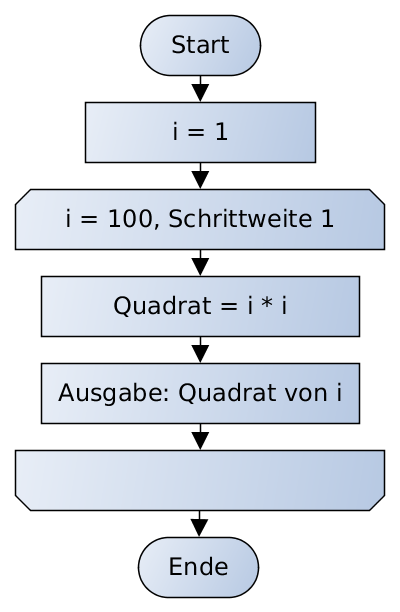
\includegraphics[scale=0.4]{pictures/lf06prog-pic/lf06prog-for-pap.png}
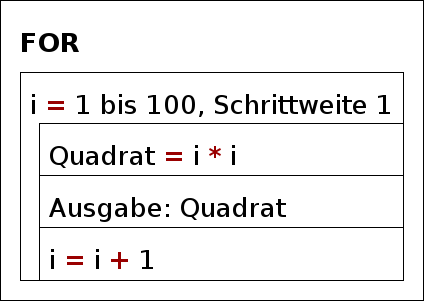
\includegraphics[scale=0.4]{pictures/lf06prog-pic/lf06prog-for-struct.png}

\subsubsection{WHILE}

% While: Fuss
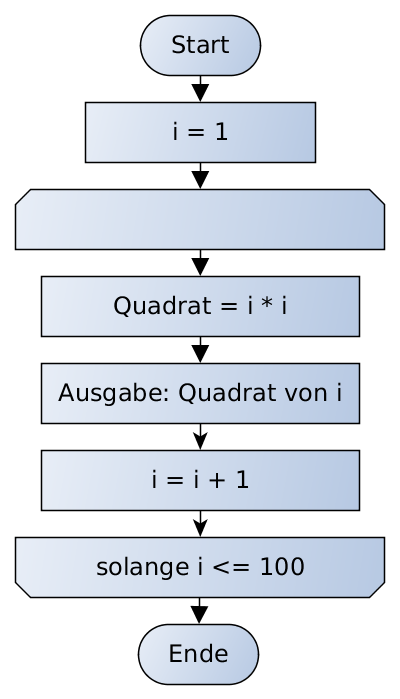
\includegraphics[scale=0.4]{pictures/lf06prog-pic/lf06prog-while-fuss-pap.png}
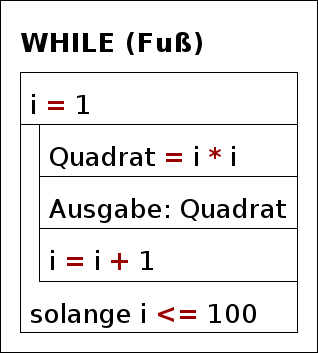
\includegraphics[scale=0.4]{pictures/lf06prog-pic/lf06prog-while-fuss-struct.png}

% While: Kopf
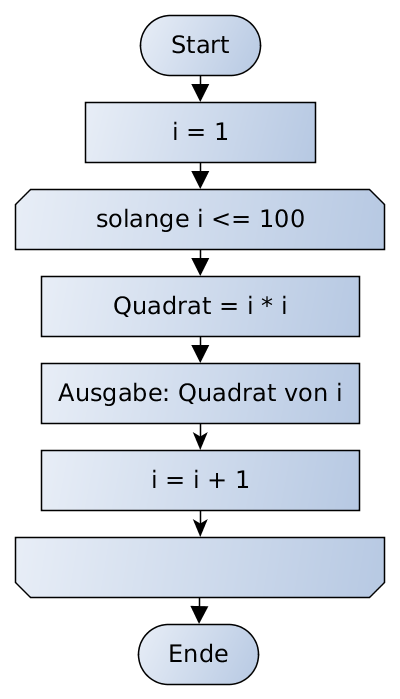
\includegraphics[scale=0.4]{pictures/lf06prog-pic/lf06prog-while-kopf-pap.png}
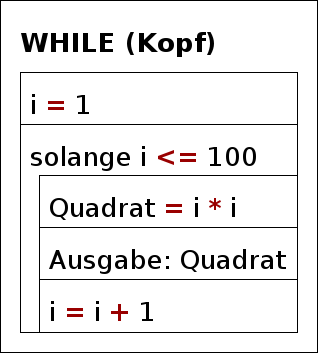
\includegraphics[scale=0.4]{pictures/lf06prog-pic/lf06prog-while-kopf-struct.png}

%%% Anfang: Verzweigung > Switch
\subsubsection{Switch-Case}
\begin{tabular}{l|l|l}

\end{tabular}
\lstinputlisting
	[caption={Ein Beispiel für Switch-Case-Anweisungen}
	\label{lst:Switch-Case},captionpos=b,language=PHP]
	{code/lf06prog-code/lf06prog-switch.case.php}

\subsubsection{Arrays}

\paragraph{Indexorientierte Arrays}~\\

\paragraph{Assoziative Arrays}~\\

%%% Ende: Verzweigung
%%%%%%%%%%%%%%%%%%%%%%%%%%%%%%%%%%%%%%%%%%%%%%%%%%%%%%%%%%%%%%%%%%%%%%%%%%%%%%%%

%%% Anfang: Aufgaben
\subsubsection{Aufgaben und Beispiele}